\documentclass[12pt,a4paper]{article}
\usepackage[utf8]{inputenc}
\usepackage{float}
\usepackage[dvips]{graphicx}
\usepackage[russian]{babel}
\usepackage[colorlinks,urlcolor=blue,citecolor=blue,linkcolor=black,menucolor=black]{hyperref}
\usepackage{color}
\usepackage{cite}
\usepackage{bm}
\usepackage{cmap}
\usepackage{indentfirst}
\usepackage{amssymb}
\usepackage{amsmath}  
\usepackage{tabularx}
\usepackage[left=2cm,right=2cm,
top=2cm,bottom=2cm,bindingoffset=0cm]{geometry}

\setcounter{tocdepth}{2}
\begin{document}
	\begin{titlepage}
		\begin{center}
			Федеральное государственное бюджетное образовательное учереждение\\
			высшего образования\\[0.5cm]
			Омский государственный университет им. Ф.М. Достоевского\\[0.5cm]
			Кафедра теоритической физики\\[2cm]
			
			Отчет о выполнении учебного задания  по <<Методам обработки массивов численных данных>>\\
			
			{\large{Исследование точки фазового перехода в двумерной модели Изинга}}\\[2cm]
		\end{center}
		
		\begin{flushright}
			Выполнил:\\ студент группы ФПБ - 603\\
			Ковалев Юрий Викторович\\[2cm]
			Заведующий кафедрой:\\
			доктор физ.-мат. наук,\\
			профессор Прудников В.В.\\*[2cm]
		\end{flushright}
		
		\begin{center}
			Омск--2019
		\end{center}
	\end{titlepage}
	\newpage
	
	\setcounter{page}{2} \tableofcontents
	\newpage
	\graphicspath{{pic/}}
	\DeclareGraphicsExtensions{.eps, .pdf}
		\section*{Введение}
	В данной работе будет исследоваться точка фазового перехода второго рода в двухмерной модели Изинга. Температуру фазового перехода будем определять с помощью метода кумулянтов Биндера.
	Поиск критической точки осуществим наложением графиков зависимости кумулянты Биндера от времени.
	Кумулянта Биндера определятся как $U = \frac{1}{2}(3 - \frac{<M^4>}{{<M^2>}^2})$, так же нам известно, что $\frac{dU}{dt} \sim (T - T_C)$, это означает , что кумулянта систем с разными размерами будет иметь точку пересечения в $T_C$, но так как рассчитанная кумулянта прерывна(расчитывается в отдельно взятых точках), вместо точки мы получим треугольник, центр тяжести которого мы выберем в качестве $T_C$. Для исследования были выбраны системы с линейными размерами $L = 128, 256, 512$
	
	\section{Этап - первичные результаты}
	Для первичного исследования критической температуры $ T_C$
	был взят интервал $T \in [1.8, 2.8]$ с шагом $\delta T = 0.02$. Для каждого линейного размера кумулянта усреднялась по 2000 конфигураций, а на время релаксации для $L = 128, 256, 512$ было выделено $1500, 900, 600$ шагов Монте-Карло $(MCS)$ соответственно. На представленных ниже графиках кумулянт мы видем,
	где локализована  $T_C$. Так же на графике можно заметить хаотичное поведение кумулянт. Объеснение этого поведения будет ниже.
	\begin{center}
	\mbox{
		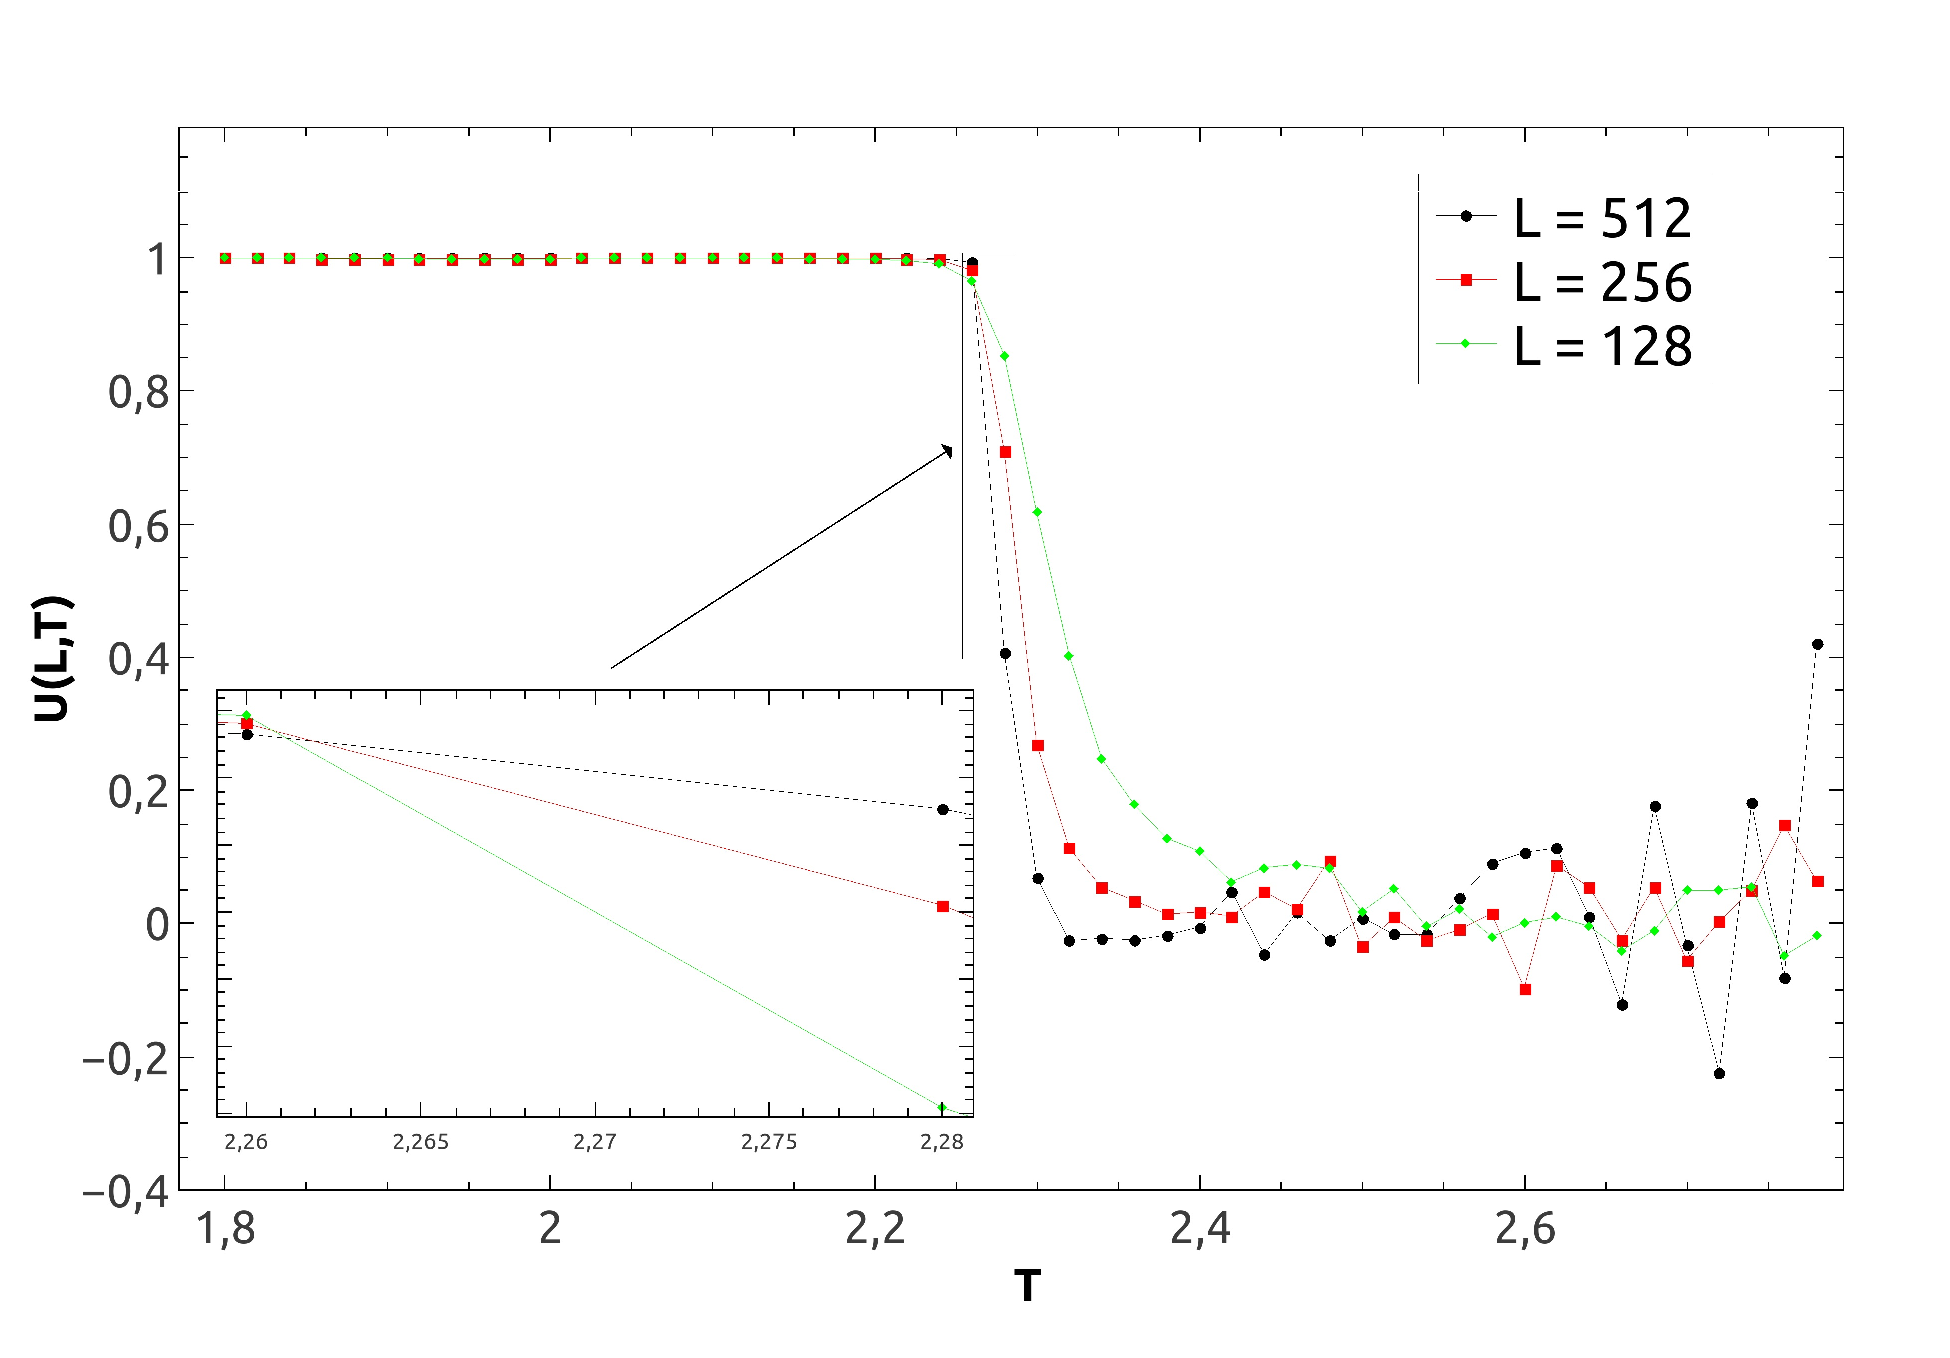
\includegraphics[scale=0.4]{U(L,T)}
	} 
	\end{center}
	\section{Этап - проверка полученных результатов}
	Неплохо было бы как то закрепить правильность полученных результатов. Мы можем это сделать, взглянув на поведение
	других характеристик системы, критическое поведение которых нам известно. И сравнить локализацию области, где проявлятся это поведение, с полученными результатами.
	Восприимчивость системы имеет пик, несовпадающий с $T_C$, в силу конечности размеров системы, но с ростом размеров системы, пик восприимчивости в нее стремиться.
	$T_p = T_C + L^{-\frac{1}{\nu}}$, где $T_p$ точка пика.
	Мы можем экстраполировать по пикам, тем самым найти найти значение $T_p$ для системы c $L = \infty$. Но размеры нашей системы велики и $L^{-\frac{1}{\nu}}$ мало, так что мы можем увидеть, что критическое поведение восприимчивости проявляется а той области, в которой и предполагалось.
	\begin{center}
	\mbox{
		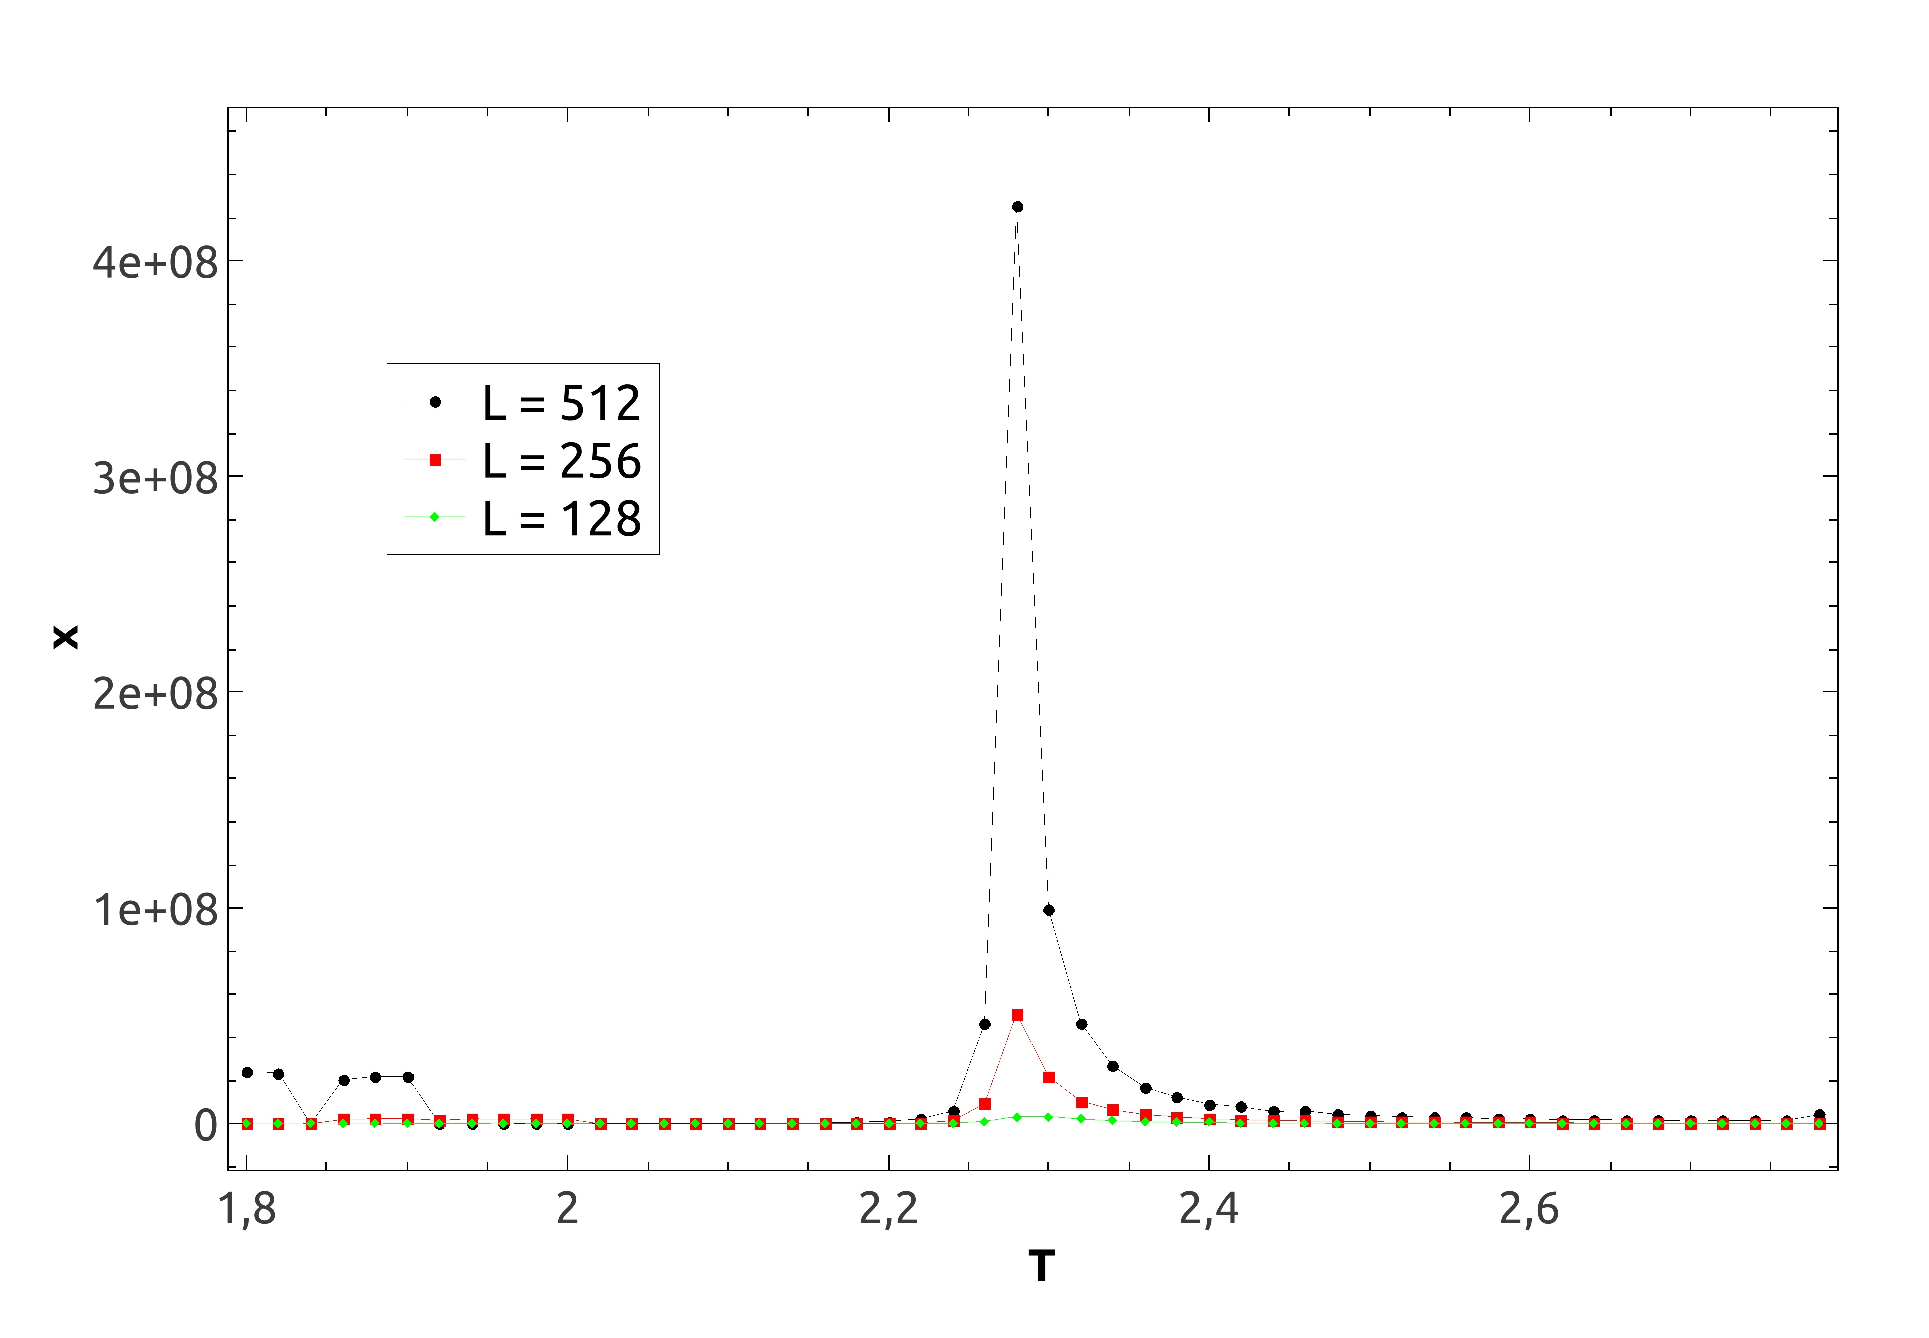
\includegraphics[scale=0.4]{chi}
	}
	\end{center} 
	Так же мы можем рассмотреть намагниченность системы.
	Как мы знаем, в $T_C$ система перестает обладать <<спонтанной намагниченостью>>. В области $T_C$ мы должны наблюдать резкий спад намагниченности системы, что мы и видим из графика
	\begin{center}
		\mbox{
			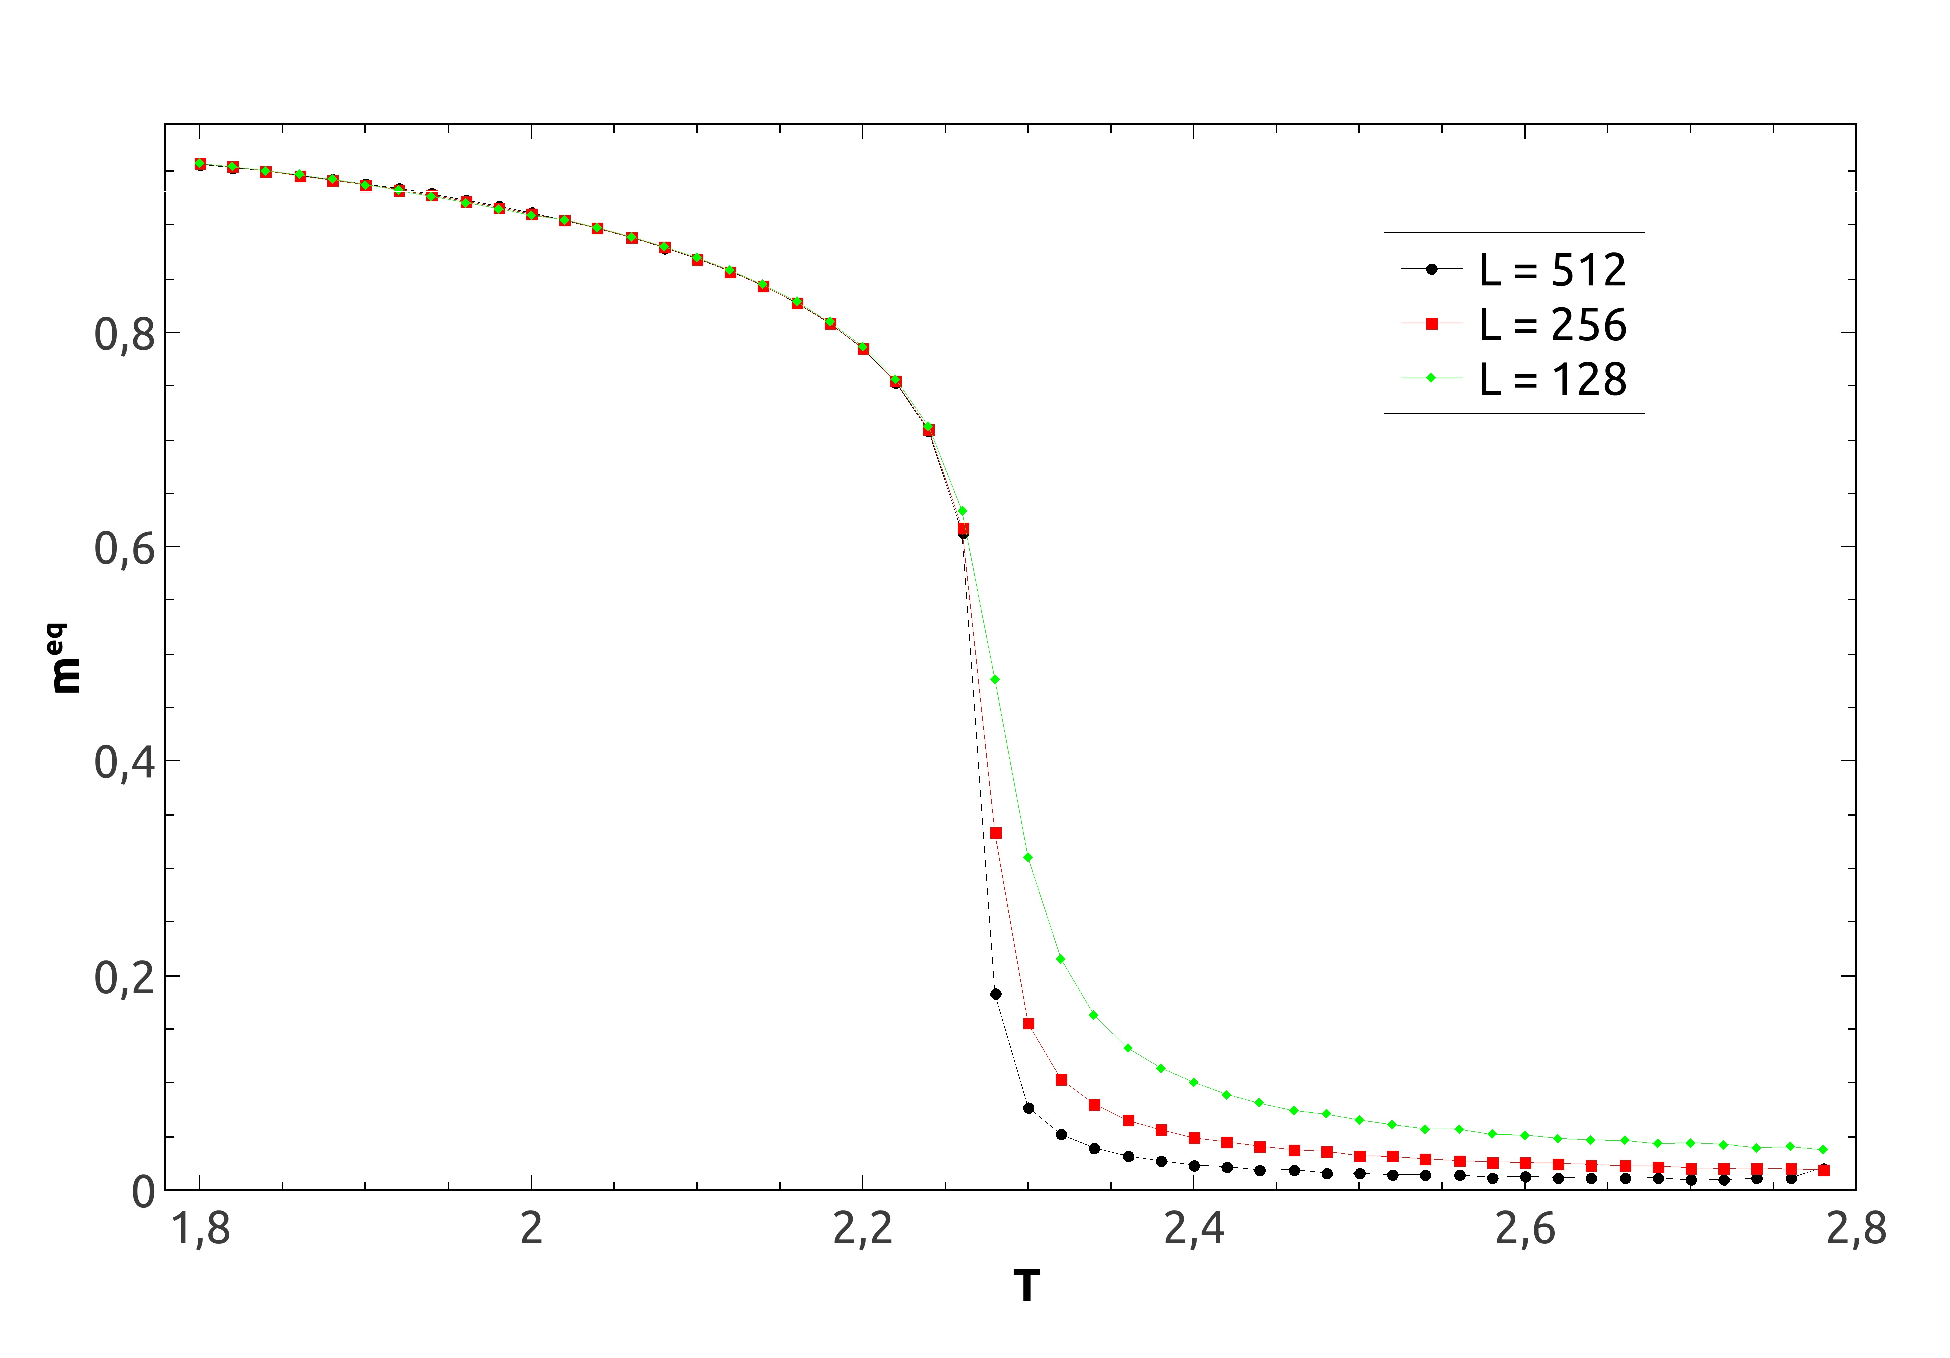
\includegraphics[scale=0.4]{meq}
		}
	\end{center}
	\section{Этап - уточнение критической температуры}
	Для дальнейшего исследования $T_C$
	был взят интервал $T \in [2.26, 2.28]$ с шагом $\delta T = 0.001$. Для каждого линейного размера кумулянта усреднялась по 2000 конфигураций, а на время релаксации для $L = 128, 256, 512$ было выделено $3000, 1800, 1200$ $(MCS)$ соответственно. На представленных ниже графикоф кумулянт мы видем,
	где локализована  $T_C$.
	\begin{center}
		\mbox{
			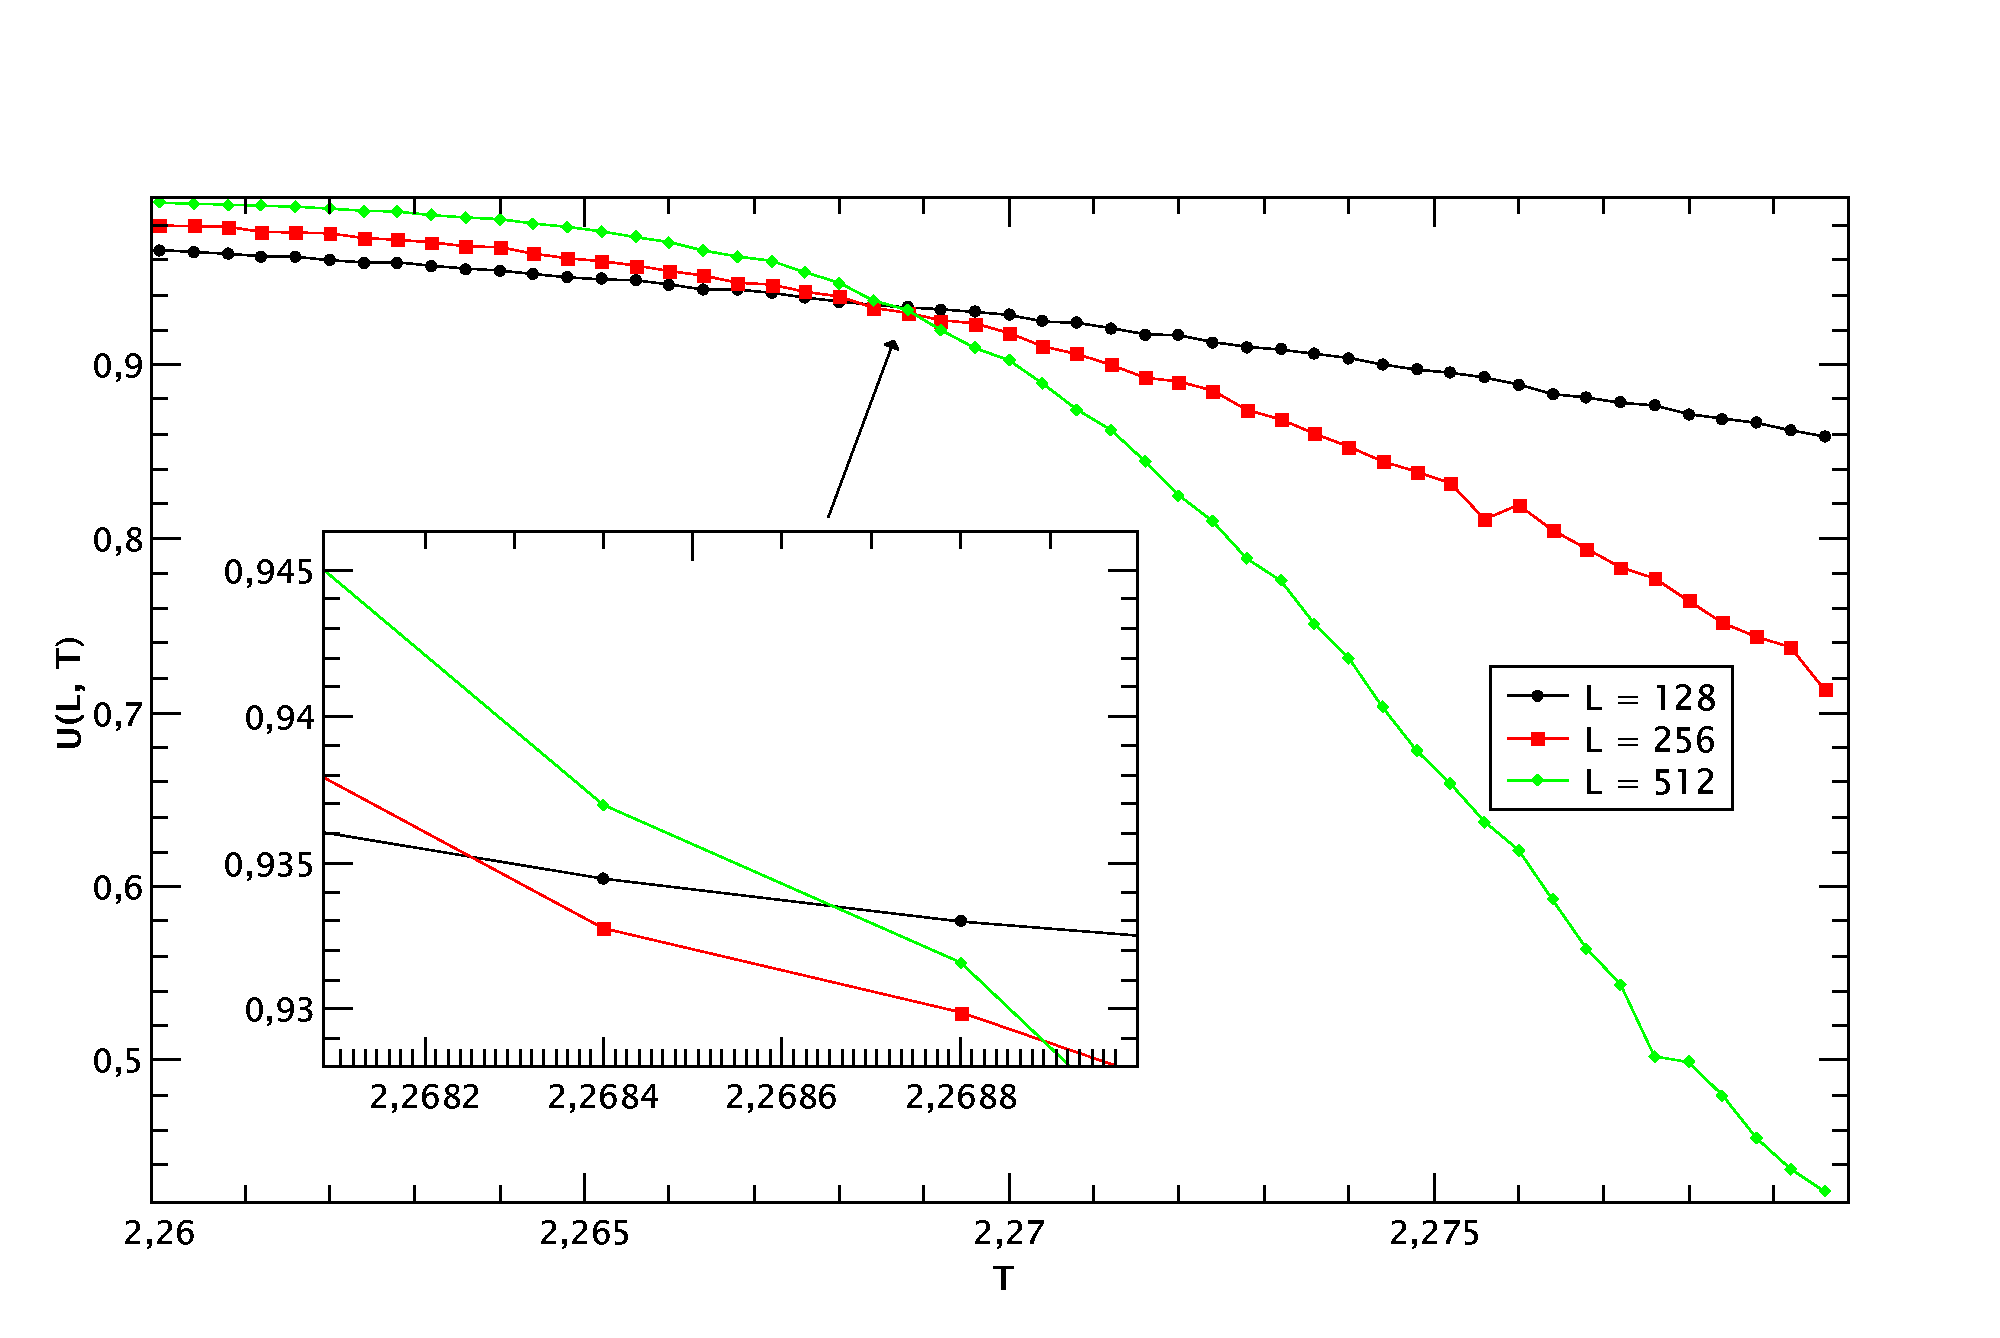
\includegraphics[scale=0.4]{kum2}
		}
	\end{center} 
	
	Теперь апроксимируем вблизи места пересечения кумулянт и окончательно получим результат.
	\begin{center}
		\mbox{
			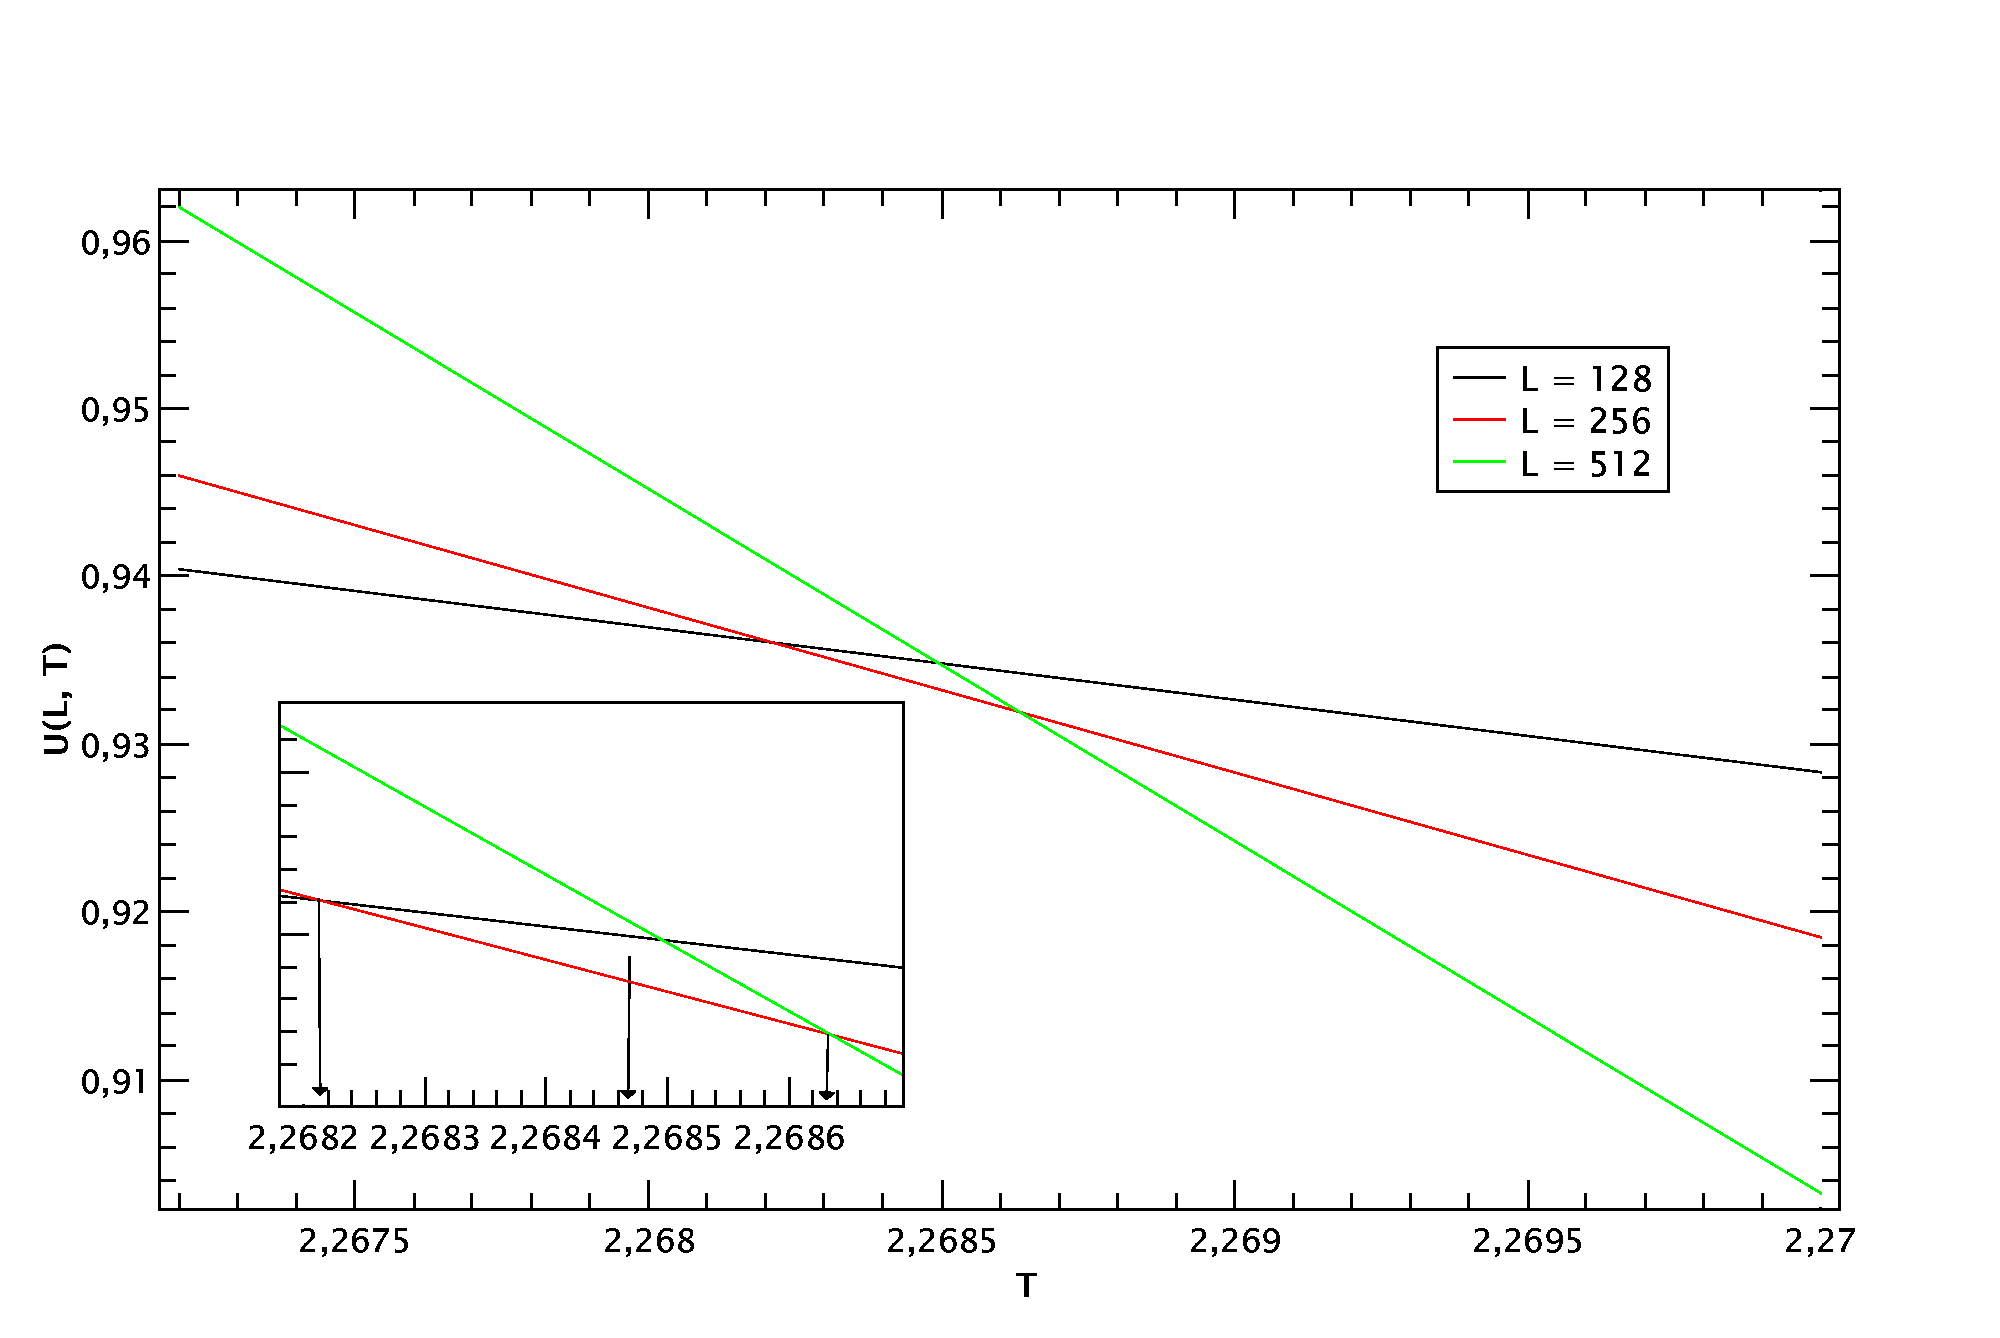
\includegraphics[scale=0.4]{AKUM}
		}
	\end{center}
	$T_C$ это центр - тяжести нашего треугольника, а в качестве погрешности возьмем половину проекции его наибольшей стороны на ось $T$.
	Итог $T_C = 2.26847(21)$
	\section{Этап - что не так ?}
	В данной работе мы не шли путем первопроходцев, а в учебных целях повторяли этот путь, поэтому мы можем сравнить наш результат с проверенным $T_C = 2.26919$. На первый взгляд исследование было проведено корректно, но, сравнивая полученный ответ с известным мы получим разницу в $0.00072$ , что совсем не укладывается в погрешность. Итог : Исследование проведено не корректно.
	И так, давайте разбираться.
	Нехватка статистики дала бы нам большую погрешность, так будем считать, что на этом фронте у нас все хорошо.
	Анализ програмного обеспечения говорит нам о том, что ошибок при написании кода допущено не было.
	Остается один вариант - начальные параметры. И это действительно оно.
	В начале отчета было сакцентировано внимание на хаотичном поведении кумулянт выше $T_C$. А еще если учесть тот факт, что исследование равновесных характеристик начинается из высокотемпературной области(области выше $T_C$), c последующим понижением температуры, то становится ясным тот факт, что для исследования было взято слишком маленькое время релаксации.
	 
	\section{Вывод и оценка масштаба трагедии}
	Несмотря на допущенную ошибку, неопытность и халатность, был получен результат, который нельзя назвать вкорне неверным.
	Если убрать вышеперечисленные недостатки, то исследование можно назвать <<успешным>>.
	
%>>>>>>>>>>>>>>>>>>>>>>>>>>>>>>>>>>>>>>>>>>>>>>>>>>>>

\newpage
\end{document}
